\chapter{Le bloc p, II~: oxygène, halogènes et gaz nobles}\label{ch:b1:p-block-16-18}

L'acide sulfurique est le produit chimique fabriqué au plus gros
tonnage~: il dissout les phosphates naturels pour les engrais, lixivie
les minerais de cuivre et d'uranium, sert au raffinage du pétrole et
remplit les batteries des voitures~; pendant un siècle, la production
d'acide sulfurique a été une mesure grossière de l'industrie d'un pays.
La majeure partie de son soufre provient aujourd'hui de l'épuration du
gaz naturel et du pétrole~; une partie est encore extraite à dos
d'homme des cratères volcaniques. Le soufre se trouve dans le \omterm{def:b1:periodicity:table}{groupe} 16,
sous l'oxygène~; les \omterm{def:b1:p-block-16-18:halogen}{halogènes} du \omterm{def:b1:periodicity:table}{groupe} 17 et les gaz nobles du
\omterm{def:b1:periodicity:table}{groupe} 18 complètent le \omterm{def:b1:periodicity:table}{bloc} p. Ce chapitre suit l'oxygène et le soufre
de l'élément à l'acide, classe les \omterm{def:b1:p-block-16-18:halogen}{halogènes} comme \omterm{def:b1:nernst:couple}{oxydants} à l'aide de
leurs \omterm{def:b1:nernst:electrode-potential}{potentiels standard}, et se termine par les composés que forment
les gaz nobles, réputés inertes.

\begin{recall}
Les \omterm{def:b1:lewis-resonance-vsepr:lewis}{schémas de Lewis}, l'extension de l'octet et les géométries VSEPR
(\cref{ch:b1:lewis-resonance-vsepr})~; les \omterm{def:b1:nernst:electrode-potential}{potentiels standard}
(\cref{ch:b1:nernst})~; la \omterm{def:b1:e-ph-diagrams:disproportionation}{dismutation} du dichlore et le \omterm{def:b1:e-ph-diagrams:e-ph-diagram}{diagramme
potentiel--pH} du chlore
(\cref{ch:b1:e-ph-diagrams})~; la catalyse (\cref{ch:b1:elementary-steps}).
Le volume scolaire (année 10) a regroupé les \omterm{def:b1:p-block-16-18:halogen}{halogènes} et les gaz nobles
en familles.
\end{recall}

\begin{omfigure}
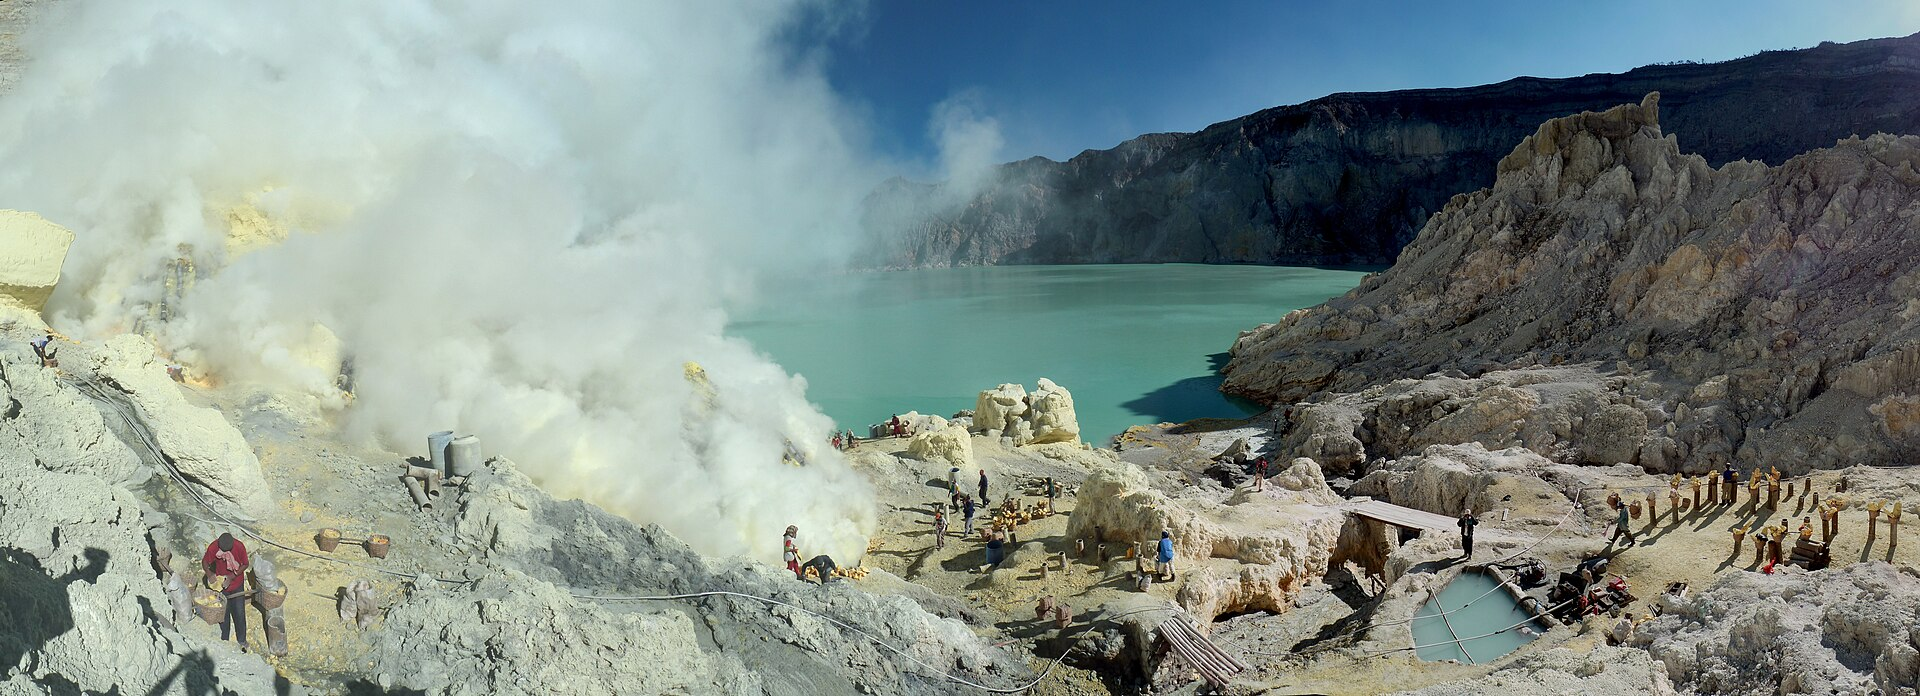
\includegraphics[width=0.78\linewidth]{images/book2/kawah-ijen.jpg}

{\small Extraction du soufre dans le cratère du volcan Kawah Ijen, en
Indonésie~: les gaz volcaniques déposent du soufre jaune autour de tuyaux,
et les mineurs le sortent dans des paniers (photographie Sémhur, CC BY-SA
4.0, Wikimedia Commons).}
\end{omfigure}

\section{Oxygène, ozone et peroxydes}

\begin{definition}[Chalcogènes]\label{def:b1:p-block-16-18:chalcogen}
Les \emph{chalcogènes}\index{chalcogene@chalcogène} sont les éléments du
\omterm{def:b1:periodicity:table}{groupe} 16
(O, S, Se, Te, Po), à six \omterm{def:b1:quantum-numbers:configuration}{électrons de valence} \textit{ns}$^2$\textit{np}$^4$.
Ils forment des composés de \omterm{def:b1:nernst:oxidation-number}{nombres d'oxydation} compris entre $-$II
(oxydes, sulfures) et $+$VI (sulfates), les plus élevés n'existant qu'à
partir du soufre.
\end{definition}

L'oxygène existe sous forme de dioxygène \ce{O2} et d'ozone \ce{O3},
molécule coudée décrite par deux \omterm{def:b1:lewis-resonance-vsepr:resonance}{formules mésomères}
(\cref{ch:b1:lewis-resonance-vsepr}). L'ozone est un \omterm{def:b1:nernst:couple}{oxydant} plus fort
que le dioxygène~: $E^\circ(\ce{O3}/\ce{O2}) = 2.07$~V
contre 1.23~V pour \ce{O2}/\ce{H2O}. Dans la haute atmosphère, il
absorbe le rayonnement ultraviolet~; près du sol, c'est un polluant. Le
peroxyde d'hydrogène, qui comporte une liaison \ce{O-O} et de l'oxygène
au degré $-$I, est à la fois \omterm{def:b1:nernst:couple}{oxydant} et \omterm{def:b1:nernst:couple}{réducteur}, et se dismute
lentement (\cref{exo:b1:nernst:12}).
% ledger: dfg:O3_g (E0 computed in figdata/bachelor-1/standard-potentials.py)

\begin{example}[Les nombres d'oxydation de l'oxygène]
L'oxygène, qui n'est dépassé en \omterm{def:b1:periodicity:electronegativity}{électronégativité} que par le fluor, est
au degré $-$II dans presque tous ses composés~: eau, oxydes, hydroxydes,
sulfates. Les exceptions découlent de la règle selon laquelle les
électrons partagés vont au partenaire le plus électronégatif et sont
répartis également entre atomes identiques. Dans le peroxyde
d'hydrogène \ce{H2O2}, H--O--O--H, chaque oxygène prend les électrons de
sa liaison \ce{O-H} mais partage le doublet \ce{O-O}~: $-$I. Dans le
superoxyde de potassium \ce{KO2}, l'ion \ce{O2-} porte une charge pour
deux atomes~: $-\frac12$ en moyenne. Dans le difluorure d'oxygène
\ce{OF2}, le fluor l'emporte dans les deux liaisons et l'oxygène est au
degré $+$II. Dans \ce{O2} et \ce{O3}, il est au degré 0. Seul le degré
$-$II est stable vis-à-vis de l'eau~; les peroxydes et les superoxydes
sont des \omterm{def:b1:nernst:couple}{oxydants}, et \ce{OF2} un agent de fluoration.
\end{example}

\section{Le soufre et l'acide sulfurique}

Le soufre, contrairement à l'oxygène, forme des cycles et des chaînes de
liaisons simples \ce{S-S}~: le soufre ordinaire est constitué de cycles
\ce{S8}. Il brûle en dioxyde de soufre, molécule coudée (angle O--S--O
de \ang{119.5}), qui peut être oxydée à son tour en trioxyde de soufre,
trigonal plan. Ce sont deux \omterm{def:b1:s-block:oxide-character}{oxydes acides}~: \ce{SO2} donne l'acide
sulfureux ($\mathrm{p}K_a$ 1.77 et 7.22), \ce{SO3} l'acide sulfurique.
% ledger: geo:SO2.aOSO, dfg:SO2_g, dfg:SO3_g

\begin{proposition}[Les étapes du procédé de contact]\label{prop:b1:p-block-16-18:contact-steps}
L'acide sulfurique est fabriqué à partir du soufre en quatre étapes~:
(1) \ce{S + O2 -> SO2}~; (2) \ce{2SO2 + O2 <=> 2SO3}, sur un \omterm{def:b1:elementary-steps:catalyst}{catalyseur}
d'oxyde de vanadium(V)~; (3) \ce{SO3 + H2SO4 -> H2S2O7} (oléum), le
trioxyde étant absorbé dans l'acide concentré~; (4)
\ce{H2S2O7 + H2O -> 2H2SO4}. Au total,
\ce{2S + 3O2 + 2H2O -> 2H2SO4}.
\end{proposition}

\begin{proof}
Chaque étape est équilibrée~; en additionnant $2\times(1)$, (2),
$2\times(3)$ et
$2\times(4)$, \ce{SO2}, \ce{SO3} et \ce{H2S2O7} se simplifient, et les
deux \ce{H2SO4} consommés à l'étape 3 sont régénérés à l'étape 4, ce
qui laisse
\ce{2S + 3O2 + 2H2O -> 2H2SO4}. L'étape 2 est thermodynamiquement très
favorable à température ambiante ($K = 10^{24.8}$ à \qty{25}{\celsius},
d'après les enthalpies libres de formation), mais extrêmement lente~:
c'est le \omterm{def:b1:elementary-steps:catalyst}{catalyseur}, actif seulement à chaud, qui la fait avancer, et
le compromis entre vitesse et taux de conversion est étudié dans le
volume de deuxième année. \ce{SO3} n'est pas absorbé directement dans
l'eau, car sa réaction avec la vapeur d'eau forme un fin brouillard de
gouttelettes d'acide qui traverse les absorbeurs.
\end{proof}
% ledger: dfg:SO2_g, dfg:SO3_g

\begin{omfigure}
\begin{tikzpicture}[font=\small, >={Stealth}, box/.style={draw, rounded corners, fill=omDef!8, align=center, minimum height=1.0cm}]
  \node[box] (b) at (0,0) {brûleur à soufre\\\ce{S + O2 -> SO2}};
  \node[box] (c) at (4.4,0) {convertisseur, \ce{V2O5}\\lits catalytiques};
  \node[box] (a) at (8.8,0) {tour d'absorption\\\ce{SO3} dans \ce{H2SO4}};
  \node[box] (d) at (8.8,-2.2) {dilution\\\ce{H2S2O7 + H2O}};
  \draw[<-, thick] (b.west) -- ++(-0.8,0) node[left] {air, S};
  \draw[->, thick] (b) -- node[above] {\ce{SO2}} (c);
  \draw[->, thick] (c) -- node[above] {\ce{SO3}} (a);
  \draw[->, thick] (a) -- node[right] {oléum} (d);
  \draw[->, thick] (d.west) -- ++(-1.2,0) node[left] {\ce{H2SO4}};
  \draw[->, thick] (d.east) -- ++(0.6,0) |- node[pos=0.25, right] {retour partiel} (a.east);
\end{tikzpicture}

{\small Le procédé de contact~: combustion du soufre, oxydation
catalytique de \ce{SO2}, absorption de \ce{SO3} dans l'acide sulfurique
concentré, et dilution de l'oléum. Une partie de l'acide retourne à
l'absorbeur.}
\end{omfigure}

\begin{proposition}[La force de l'acide sulfurique]\label{prop:b1:p-block-16-18:sulfuric-strength}
Dans l'eau, la première acidité de l'acide sulfurique est forte
(totale), la seconde faible~: $\mathrm{p}K_a(\ce{HSO4-}/\ce{SO4^2-}) = 1.99$.
Une solution à
\qty{0.010}{mol/L} n'est donc ni à pH 1.70 (deux protons) ni à 2.00 (un
seul), mais entre les deux.
\end{proposition}

\begin{proof}
\ce{H2SO4}, qui porte sur le soufre deux oxygènes dépourvus
d'hydrogène, est un \omterm{def:b1:p-block-13-15:oxoacid}{oxoacide} plus fort que \ce{H3O+}~: il est nivelé
(\cref{ch:b1:predominant-reaction}).
\ce{HSO4-}, déjà négatif, retient davantage son proton~: son
$\mathrm{p}K_a$,
calculé à partir des enthalpies libres de formation, vaut 1.99. Pour
$C = 0.010$~:
$[\ce{H3O+}] = C + x$, $[\ce{HSO4-}] = C - x$, $[\ce{SO4^2-}] = x$, avec
$x(C + x)/(C - x) = 10^{-1.99}$~; en résolvant, $x = \qty{4.2e-3}{mol/L}$
et
$\mathrm{pH} = -\log(0.0142) = 1.85$.
\end{proof}
% ledger: dfg:HSO4-_ao, dfg:SO42-_ao

L'acide sulfurique concentré est aussi un puissant déshydratant (il
carbonise le sucre en lui arrachant les éléments de l'eau) et, à chaud,
un \omterm{def:b1:nernst:couple}{oxydant}. Sa dilution dégage beaucoup de chaleur~: on verse toujours
l'acide dans l'eau, jamais l'inverse. La majeure partie du soufre
mondial, environ 84 millions de tonnes en 2025, est récupérée à partir
du sulfure d'hydrogène du gaz naturel et des effluents de raffinerie, et
finit pour l'essentiel en acide sulfurique.
% ledger: usgs:S-world-2025

\begin{method}[Bilan de matière à travers le procédé de contact]\label{met:b1:p-block-16-18:contact-balance}
\begin{enumerate}
  \item Utiliser l'équation globale~: un \ce{H2SO4} par atome de S.
  \item Corriger du taux de conversion de l'étape 2 (la fraction de
        \ce{SO2} oxydée) et des pertes à l'absorption.
  \item Pour l'air~: calculer le \ce{O2} nécessaire (trois demis par S)
        et diviser par sa fraction dans l'air.
\end{enumerate}
\end{method}

\begin{example}[Une usine qui brûle mille tonnes de soufre par jour]
Une usine brûle \qty{1000}{t} de soufre par jour, convertit
\qty{99.0}{\percent} du \ce{SO2} et absorbe \qty{99.9}{\percent} du
\ce{SO3}. Alors
$n(\ce{S}) = \num{1000e6}/32.1 = \qty{3.12e7}{mol}$ et
$n(\ce{H2SO4}) = \num{3.12e7} \times 0.990 \times 0.999
= \qty{3.08e7}{mol}$, soit $\num{3.08e7} \times \qty{98.1}{g}
= \qty{3020}{t}$ d'acide par jour. Le \qty{1.0}{\percent} non converti
sort sous forme de \ce{SO2}~: \qty{3.1e5}{mol}, soit \qty{20}{t} par
jour, qu'il faut retirer des gaz de queue. Le dioxygène nécessaire vaut
$1.5 \times \num{3.12e7} =
\qty{4.67e7}{mol}$~; l'air, à \qty{21}{\percent} de \ce{O2}, représente
\qty{2.23e8}{mol}, soit $V = nRT/p = \qty{5.5e6}{m^3}$ par jour à
\qty{25}{\celsius} et \qty{1}{bar}, avant l'excès que l'usine insuffle
réellement.
\end{example}
% ledger: air:O2

\section{Les halogènes}

\begin{definition}[Halogènes]\label{def:b1:p-block-16-18:halogen}
Les \emph{halogènes}\index{halogene@halogène} sont les éléments du
\omterm{def:b1:periodicity:table}{groupe} 17 (F, Cl,
Br, I, At), à sept \omterm{def:b1:quantum-numbers:configuration}{électrons de valence} \textit{ns}$^2$\textit{np}$^5$.
Ils existent sous forme de molécules diatomiques \ce{X2} et forment des
ions halogénure \ce{X-}.
\end{definition}

\begin{omfigure}
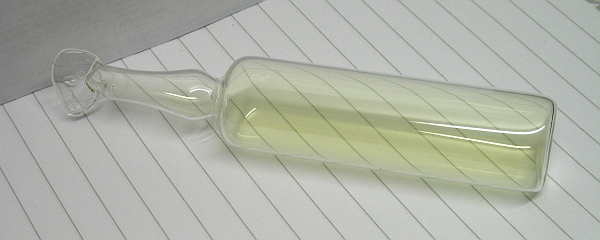
\includegraphics[height=2.9cm]{images/book2/chlorine.jpg}\hspace{0.5em}%
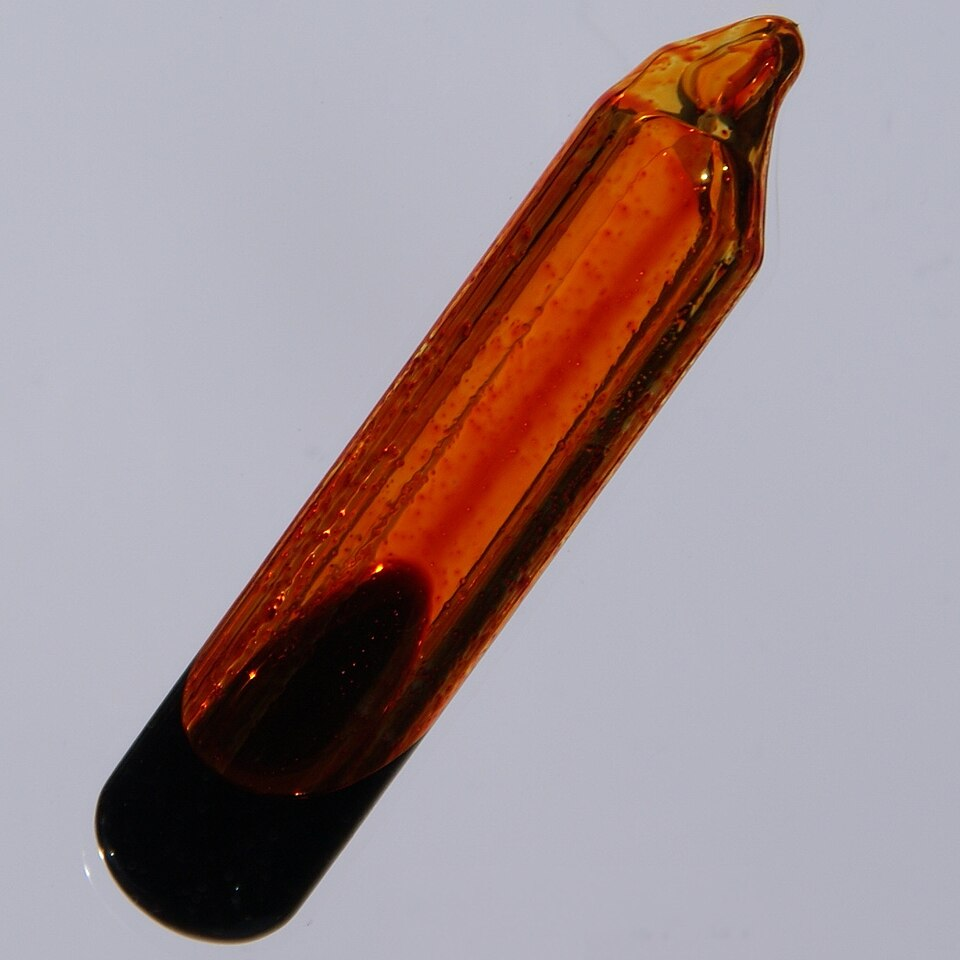
\includegraphics[height=2.9cm]{images/book2/bromine.jpg}\hspace{0.5em}%
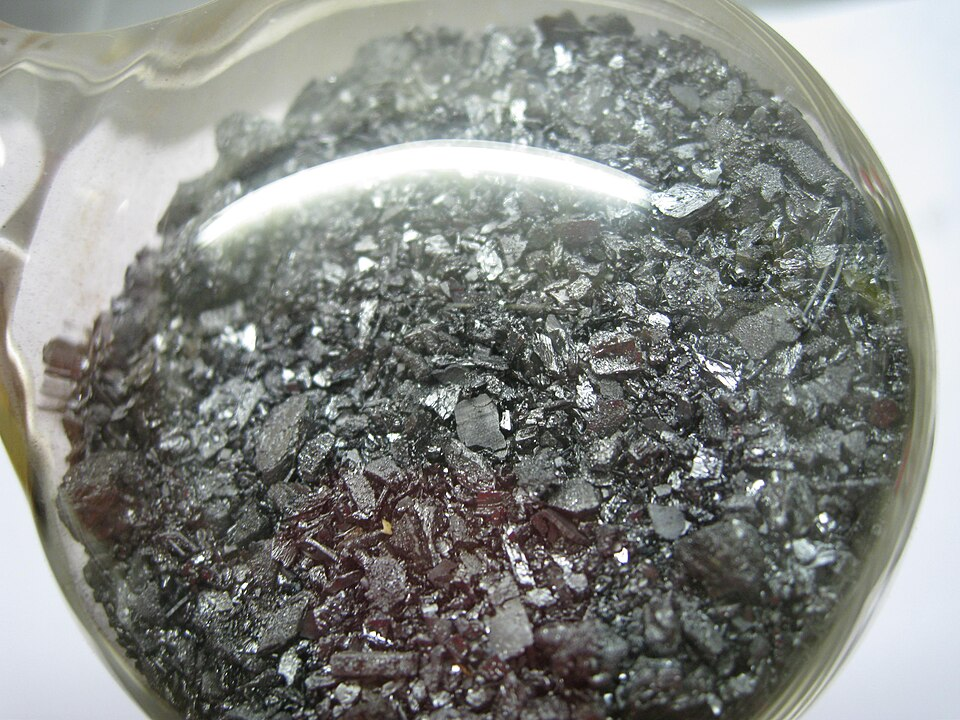
\includegraphics[height=2.9cm]{images/book2/iodine.jpg}

{\small Le dichlore, gaz jaune-vert pâle (W. Oelen, CC BY-SA 3.0)~; le
dibrome, liquide rouge sombre aux vapeurs orangées (Jurii, CC BY 3.0)~;
le diiode, \omterm{def:b1:crystals-metals:crystal}{cristaux} gris-noir à l'éclat métallique (Dnn87, CC BY 3.0).
Le dichlore et le dibrome sont scellés dans des ampoules de verre. Toutes
les images proviennent de Wikimedia Commons.}
\end{omfigure}

\begin{proposition}[Pouvoir oxydant des halogènes]\label{prop:b1:p-block-16-18:halogen-oxidising-order}
Les \omterm{def:b1:p-block-16-18:halogen}{halogènes} sont des \omterm{def:b1:nernst:couple}{oxydants} dont la force diminue en descendant le
groupe~:
$E^\circ(\ce{F2}/\ce{F-}) = 2.89$~V, \ce{Cl2}/\ce{Cl-} 1.36~V,
\ce{Br2}/\ce{Br-} 1.08~V, \ce{I2}/\ce{I-} 0.53~V. Chaque \omterm{def:b1:p-block-16-18:halogen}{halogène} oxyde
les ions halogénure situés au-dessous de lui dans le groupe.
\end{proposition}

\begin{proof}
Les valeurs proviennent des enthalpies libres de formation des ions
halogénure (\cref{ch:b1:nernst}). D'après la règle du gamma, \ce{X2}
oxyde \ce{Y-} lorsque le couple \ce{X2}/\ce{X-} est situé au-dessus de
\ce{Y2}/\ce{Y-}~: par exemple
\ce{Cl2 + 2Br- -> 2Cl- + Br2}, $\log K = 2(1.36 - 1.08)/0.059 = 9.5$.
En descendant le groupe, les atomes grossissent~; leur affinité pour un
électron supplémentaire et l'hydratation des ions halogénure, qui
favorise les plus petits, diminuent, et le potentiel avec elles.
\end{proof}
% ledger: dfg:F-_ao, dfg:Cl-_ao, dfg:Br-_ao, dfg:I-_ao

\begin{omfigure}
\begin{tikzpicture}
\begin{axis}[
  ybar, width=0.62\linewidth, height=5.0cm, ymin=0, ymax=3.3,
  symbolic x coords={F,Cl,Br,I}, xtick=data,
  xticklabels={\ce{F2}/\ce{F-}, \ce{Cl2}/\ce{Cl-}, \ce{Br2}/\ce{Br-}, \ce{I2}/\ce{I-}},
  ylabel={$E^\circ$ (V)}, bar width=16pt, nodes near coords,
  every node near coord/.append style={font=\scriptsize},
  tick label style={font=\small}, label style={font=\small}, enlarge x limits=0.2]
\addplot[fill=omThm!40, draw=omThm] coordinates {(F,2.89) (Cl,1.36) (Br,1.08) (I,0.53)};
\end{axis}
\end{tikzpicture}

{\small \omterm{def:b1:nernst:electrode-potential}{Potentiels standard} des couples halogène--halogénure à
\qty{25}{\celsius}, calculés à partir d'enthalpies libres tabulées~: le
pouvoir \omterm{def:b1:nernst:couple}{oxydant} diminue régulièrement en descendant le groupe.}
\end{omfigure}

Les halogénures d'hydrogène sont tous des acides dans l'eau, mais
\ce{HF} est faible ($\mathrm{p}K_a$ 3.16) alors que \ce{HCl}, \ce{HBr} et
\ce{HI} sont forts~: la liaison
\ce{H-F} est très forte et le petit ion fluorure est retenu par de
fortes \omterm{def:b1:intermolecular-forces-solvents:hbond}{liaisons hydrogène}. Le fluor est l'élément le plus
électronégatif et l'\omterm{def:b1:nernst:couple}{oxydant} le plus fort de la table~; on ne l'obtient
que par électrolyse. Les \omterm{def:b1:p-block-13-15:oxoacid}{oxoacides} du chlore --- acide hypochloreux
\ce{HClO}, acide chlorique \ce{HClO3}, acide perchlorique \ce{HClO4} ---
sont d'autant plus forts qu'ils comptent plus d'oxygènes dépourvus
d'hydrogène, comme tous les \omterm{def:b1:p-block-13-15:oxoacid}{oxoacides} (\cref{def:b1:p-block-13-15:oxoacid})~;
leurs relations avec l'ion chlorure et le dichlore ont été cartographiées
au \cref{ch:b1:e-ph-diagrams}.
% ledger: dfg:HF_ao, dfg:F-_ao

\begin{omfigure}
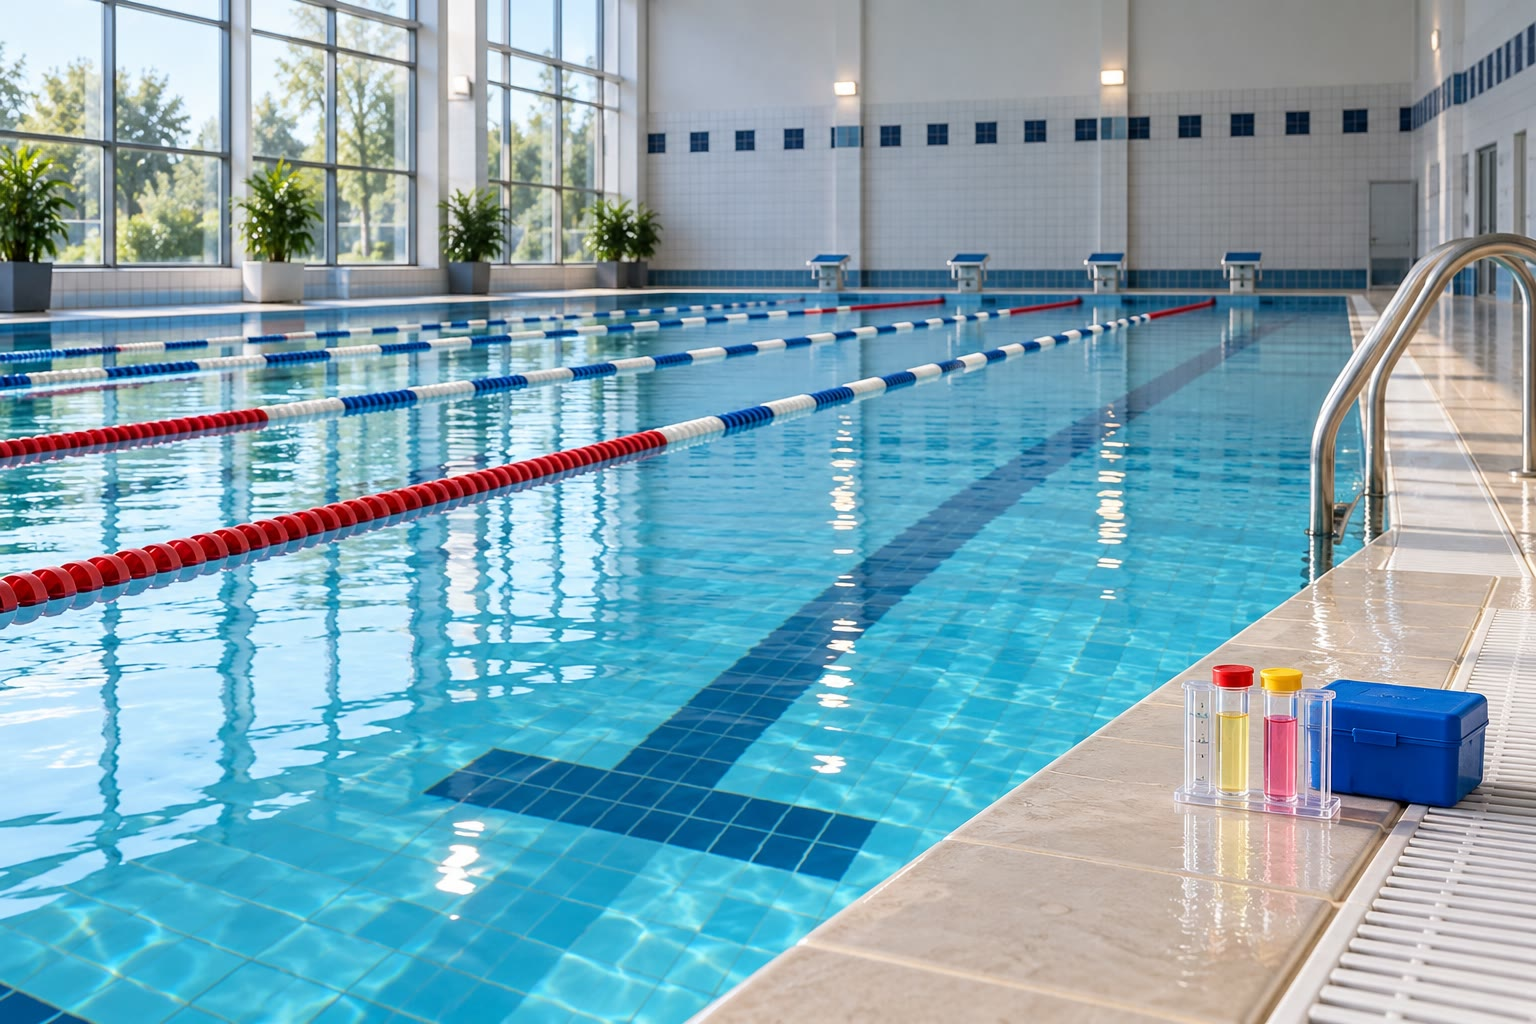
\includegraphics[width=0.55\linewidth]{images/book2/ai/b1-28-swimming-pool.jpg}

{\small Une piscine publique et sa trousse d'analyse de l'eau~: le chlore
dissous sous forme d'acide hypochloreux est contrôlé plusieurs fois par
jour.}
\end{omfigure}

\begin{definition}[Composés interhalogénés]\label{def:b1:p-block-16-18:interhalogen}
Un \emph{composé interhalogéné}\index{compose interhalogene@composé interhalogéné}
est un composé de deux \omterm{def:b1:p-block-16-18:halogen}{halogènes} différents~: \ce{ICl}, \ce{BrF3},
\ce{ClF3}, \ce{IF7}. L'\omterm{def:b1:p-block-16-18:halogen}{halogène} le plus gros et le moins électronégatif
est l'\omterm{def:b1:complexation:complex}{atome central}, avec un octet étendu à partir de \ce{ClF3}.
\end{definition}

\begin{inthelab}[Manipuler les halogènes]
Le dichlore est toxique et ne se prépare qu'en petites quantités sous la
hotte~; le dibrome brûle la peau et ses vapeurs attaquent les poumons~:
on l'emploie dilué, sous la hotte, avec gants et lunettes, une solution
de thiosulfate de sodium à portée de main pour détruire les
éclaboussures
(\ce{4Br2 + S2O3^2- + 5H2O -> 8Br- + 2SO4^2- + 10H+}). Le diiode est le
plus inoffensif des trois, mais il tache et se sublime~; on le conserve
dans un flacon fermé.
\end{inthelab}

\section{Les gaz nobles et leurs composés}

Les gaz nobles (He, Ne, Ar, Kr, Xe, Rn) ont des couches de valence
pleines et les énergies d'ionisation les plus élevées de leur \omterm{def:b1:periodicity:table}{période}
(\cref{ch:b1:periodicity}). Longtemps crus inertes, les plus lourds,
dont les électrons externes sont moins fortement retenus, réagissent
bel et bien avec les éléments les plus électronégatifs~: le xénon donne
\ce{XeF2}, \ce{XeF4}, \ce{XeF6} et des oxydes. Leurs géométries suivent
les règles VSEPR, avec des \omterm{def:b1:lewis-resonance-vsepr:lewis}{doublets non liants} sur le xénon.

\begin{example}[Pourquoi le xénon, et pas l'argon]
Les \omterm{def:b1:periodicity:ionisation-energy}{énergies de première ionisation} des gaz nobles diminuent en
descendant le groupe~: He
24.59, Ne 21.56, Ar 15.76, Kr 14.00, Xe 12.13, Rn 10.75~eV. Celle du
dioxygène, \ce{O2 -> O2+ + e-}, vaut 12.07~eV, presque autant que celle
du xénon. Un \omterm{def:b1:nernst:couple}{oxydant} assez fort pour arracher un électron à \ce{O2}, en
donnant le cation dioxygényle \ce{O2+}, devrait donc oxyder aussi le
xénon, mais pas l'argon, qui retient son électron 3.7~eV plus
fortement. Le xénon réagit effectivement avec l'hexafluorure de platine
\ce{PtF6}, \omterm{def:b1:nernst:couple}{oxydant} très puissant, en donnant un solide de composition
globale \ce{XePtF6}, et avec le fluor lui-même, qui donne les fluorures
de xénon du tableau ci-dessous. Le radon, plus facile encore à ioniser,
est trop radioactif pour qu'on puisse étudier beaucoup sa chimie.
\end{example}
% ledger: ie:He, ie:Ne, ie:Ar, ie:Kr, ie:Xe, ie:Rn, ie:O2, lit:XePtF6

\begin{omfigure}
\begin{tabular}{llll}
\hline
molécule & doublets de l'\omterm{def:b1:complexation:complex}{atome central} & géométrie & angle mesuré \\
\hline
\ce{SO2} & 2 domaines liants + 1 non liant & coudée & \ang{119.5} \\
\ce{SF6} & 6 liants & octaédrique & \ang{90} \\
\ce{ClF3} & 3 liants + 2 non liants & en T & \ang{87.5} \\
\ce{XeF2} & 2 liants + 3 non liants & linéaire & \ang{180} \\
\ce{XeF4} & 4 liants + 2 non liants & plan carré & \ang{90} \\
\hline
\end{tabular}

\smallskip
{\small Géométries de quelques molécules du \omterm{def:b1:periodicity:table}{bloc} p à octet étendu ou à
\omterm{def:b1:lewis-resonance-vsepr:lewis}{doublets non liants} (angles mesurés lorsqu'ils sont disponibles). Les
\omterm{def:b1:lewis-resonance-vsepr:lewis}{doublets non liants} de \ce{XeF2} occupent les trois positions
équatoriales d'une bipyramide trigonale, ce qui laisse la molécule
linéaire.}
% ledger: geo:SO2.aOSO, geo:SF6.aFSF, geo:ClF3.aFClF, geo:XeF2.aFXeF
\end{omfigure}

L'argon, qui représente près d'un pour cent de l'air, protège les
matériaux réactifs au laboratoire et en soudage~; l'hélium, tiré du gaz
naturel, refroidit les aimants supraconducteurs, comme ceux des
spectromètres de RMN (\cref{ch:b1:structure-spectroscopy}).
% ledger: air:Ar

\section{Exercices}

\begin{exercise}[$\star$]\label{exo:b1:p-block-16-18:1}
Donner le \omterm{def:b1:nernst:oxidation-number}{nombre d'oxydation} du soufre dans \ce{H2S}, \ce{S8}, \ce{SO2},
\ce{SO3^2-}, \ce{SO4^2-}, \ce{S2O3^2-} (en moyenne) et \ce{H2S2O7}.
\end{exercise}

\begin{exercise}[$\star$]\label{exo:b1:p-block-16-18:2}
Lesquelles de ces réactions ont lieu~: dichlore et iodure de
potassium~; diiode et bromure de sodium~; dibrome et chlorure de
sodium~; dichlore et bromure de sodium~? Écrire celles qui se
produisent.
\end{exercise}

\begin{exercise}[$\star$]\label{exo:b1:p-block-16-18:3}
Dessiner les \omterm{def:b1:lewis-resonance-vsepr:lewis}{schémas de Lewis} de \ce{SO2}, \ce{SO3} et \ce{O3}, avec
leurs \omterm{def:b1:lewis-resonance-vsepr:resonance}{formules mésomères}, et donner leurs géométries.
\end{exercise}

\begin{exercise}[$\star$]\label{exo:b1:p-block-16-18:4}
Écrire les réactions de \ce{SO2} et de \ce{SO3} avec l'eau et avec
l'hydroxyde de sodium.
\end{exercise}

\begin{exercise}[$\star\star$]\label{exo:b1:p-block-16-18:5}
Calculer le pH de l'acide fluorhydrique à \qty{0.10}{mol/L} et le
comparer à celui de l'acide chlorhydrique à la même concentration.
Expliquer la différence.
\end{exercise}

\begin{exercise}[$\star\star$]\label{exo:b1:p-block-16-18:6}
Prévoir par la méthode VSEPR les géométries de \ce{BrF5}, \ce{IF7}
(sept \omterm{def:b1:lewis-resonance-vsepr:lewis}{doublets liants}, bipyramide pentagonale), \ce{ICl4-} et \ce{XeO3}.
\end{exercise}

\begin{exercise}[$\star\star$]\label{exo:b1:p-block-16-18:7}
Calculer la constante de \ce{Cl2 + 2I- -> 2Cl- + I2} et dire pourquoi
l'eau de chlore bleuit un papier imprégné d'iodure et d'amidon.
\end{exercise}

\begin{exercise}[$\star\star$]\label{exo:b1:p-block-16-18:8}
Montrer que l'ozone peut oxyder les ions iodure en diiode et écrire la
réaction en milieu acide. Pourquoi s'en sert-on pour doser l'ozone~?
\end{exercise}

\begin{exercise}[$\star\star$]\label{exo:b1:p-block-16-18:9}
L'acide sulfurique concentré carbonise le saccharose, \ce{C12H22O11}.
Écrire la \omterm{def:b1:alcohol-activation:dehydration}{déshydratation} en carbone et calculer la masse de carbone
obtenue à partir de \qty{10.0}{g} de sucre.
\end{exercise}

\begin{exercise}[$\star\star\star$]\label{exo:b1:p-block-16-18:10}
Calculer le pH de l'acide sulfurique à \qty{0.10}{mol/L} en tenant compte
de la seconde acidité ($\mathrm{p}K_a = 1.99$). Quelle contribution la
seconde acidité apporte-t-elle~?
\end{exercise}

\begin{exercise}[$\star\star\star$]\label{exo:b1:p-block-16-18:11}
Expliquer à l'aide des potentiels pourquoi le fluor ne peut être
préparé en \omterm{def:b1:nernst:couple}{oxydant} l'ion fluorure par aucun \omterm{def:b1:nernst:couple}{oxydant} chimique en solution
aqueuse, et pourquoi il doit être obtenu par électrolyse d'un fluorure
fondu, et non d'une solution aqueuse.
\end{exercise}

\begin{exercise}[$\star\star\star$]\label{exo:b1:p-block-16-18:12}
Le diiode n'est que peu soluble dans l'eau, mais se dissout dans une
solution d'iodure de potassium sous forme d'ion triiodure \ce{I3-}. À
l'aide des enthalpies libres de formation de
\ce{I2(aq)} ($\Delta_f G^\circ = \qty{16.40}{kJ/mol}$), de \ce{I-}
($-51.57$)
et de \ce{I3-} ($-51.4$), calculer la constante de \ce{I2 + I- <=> I3-}.
\end{exercise}

\section{Problème~: une tonne de soufre}

\begin{problem}[{Problème du week-end --- la combustion du soufre,
l'oxydation catalytique du dioxyde de soufre, l'absorption et l'oléum,
la seconde acidité de l'acide sulfurique, et la masse d'acide fabriquée
à partir d'une tonne de soufre}]
\label{pb:b1:p-block-16-18:1}
Une usine d'acide sulfurique brûle du soufre récupéré à partir du gaz
naturel. Masses molaires
(\unit{g/mol})~: S 32.1, \ce{O2} 32.0, \ce{SO2} 64.1, \ce{SO3} 80.1,
\ce{H2SO4} 98.1, \ce{H2O} 18.0~; l'air contient \qty{21}{\percent} de
\ce{O2} en volume~; $\mathrm{p}K_a(\ce{HSO4-}) = 1.99$~; $R =
\qty{8.314}{J/(K.mol)}$.

\medskip
\noindent\textbf{Partie I --- La combustion du soufre.}
\begin{enumerate}
  \item Donner le \omterm{def:b1:nernst:oxidation-number}{nombre d'oxydation} de S dans S, \ce{SO2}, \ce{SO3} et
        \ce{H2SO4}.
  \item Écrire la combustion du soufre.
  \item Dessiner le \omterm{def:b1:lewis-resonance-vsepr:lewis}{schéma de Lewis} de \ce{SO2} et prévoir sa géométrie.
  \item Calculer la quantité de matière de soufre dans une tonne.
  \item Calculer le volume d'air (\qty{25}{\celsius}, \qty{1}{bar})
        nécessaire à la seule combustion.
  \item Pourquoi refroidit-on le gaz issu du brûleur avant le
        convertisseur~?
\end{enumerate}

\medskip
\noindent\textbf{Partie II --- L'oxydation catalytique.}
\begin{enumerate}[resume]
  \item Écrire l'oxydation de \ce{SO2} en \ce{SO3}.
  \item Sa constante à \qty{25}{\celsius} vaut environ $10^{24.8}$.
        Pourquoi faut-il néanmoins un \omterm{def:b1:elementary-steps:catalyst}{catalyseur}~?
  \item Quel est le rôle de l'oxyde de vanadium(V), dans le langage du
        \cref{ch:b1:elementary-steps}~?
  \item Dessiner la géométrie de \ce{SO3}.
  \item Pourquoi utilise-t-on un excès d'air~?
  \item Quelle fraction de \ce{SO2} est perdue si le taux de conversion
        vaut \qty{99.7}{\percent}~?
\end{enumerate}

\medskip
\noindent\textbf{Partie III --- L'absorption.}
\begin{enumerate}[resume]
  \item Écrire l'absorption de \ce{SO3} dans l'acide sulfurique.
  \item Pourquoi \ce{SO3} n'est-il pas absorbé directement dans l'eau~?
  \item Écrire la dilution de l'oléum.
  \item Écrire l'équation globale du procédé.
  \item Calculer la masse d'eau consommée par tonne de soufre.
  \item Pourquoi faut-il verser l'acide dans l'eau et jamais
        l'inverse~?
\end{enumerate}

\medskip
\noindent\textbf{Partie IV --- L'acide.}
\begin{enumerate}[resume]
  \item Calculer le pH d'une solution d'acide sulfurique à
        \qty{0.050}{mol/L} en tenant compte de la seconde acidité.
  \item Calculer la masse d'acide sulfurique pour un \omterm{def:b1:extent-q-and-k:fractional-extent}{rendement} global de
        \qty{99.5}{\percent}.
  \item Le monde a produit environ \qty{84}{Mt} de soufre en 2025. Quelle
        masse d'acide sulfurique en tirerait-on si tout était converti~?
  \item Donner la masse d'acide sulfurique que l'on peut obtenir à partir
        d'une tonne de soufre (conversion complète).
\end{enumerate}
\end{problem}
